\noindent
\graphicspath{{./18-07/Images/}} 
%%%%%%%%%%%%%%%%
% Page de gauche
%%%%%%%%%%%%%%%%
\begin{minipage}[t][\textheight][t]{0.33\textwidth}
    \colorbox{StrongBlue}{
        \parbox[c][\textheight][c]{\textwidth}{ 
            \color{OffWhite} 
            \begin{center}
                \begin{minipage}[t][0.6\textheight][c]{0.8\textwidth}
                    {\huge \textbf{Samedi 18 Juillet}}\\
                    \normalsize
                    \begin{center}
                        \begin{tabular}{@{} l @{\hspace{0.5cm}} l @{}}
                            Abri de départ : &\hfill Pornichet \\ 
                            Abri d'arrivée : &\hfill L'Herbaudière \\ 
                            Distance : &\hfill 10 Millaes nautiques \\ 
                            Départ : &\hfill  \\ 
                            Durée : &\hfill 4 Heures \\ 
                            Arrivée prévue : &\hfill  \\ 
                            Lever soleil 
\includegraphics[width=8px,height=8px]{../../Pictos/soleil_OffWhite.png} : &\hfill 06 h 31 \\ 
                            Coucher soleil 
\includegraphics[width=8px,height=8px]{../../Pictos/lune_OffWhite.png} : &\hfill 21 h 58 \\ 
                            \\
                            Abris replis : &  \\
                                    & • Pornichet \\
                                    & • La Gravette \\
                                    & • Pornic \\
                                    & • L'Herbaudière \\                     
                                
                        \end{tabular}
                    \end{center}
                    
                \end{minipage}%
                
                \begin{minipage}[t][0.4\textheight][t]{\textwidth}
                    \begin{center}
    {\large \textit{Marées \textbf{Pornichet}}}\\ \vspace{0.5em}
    
    \renewcommand{\arraystretch}{1.40} % Adjust the row height by a factor of 1.4

    \begin{tabular}{ |C{5em}|c|C{4em}|C{4em}| } \hline
        & Coef & Heure & Hauteur\\ \hline
        BM & \multirow{2}{1em}{91}  & 08 h 01 & 5.20 m\\ \cline{1-1} \cline{3-4}
        PM &                        & 14 h 35 & 1.00 m\\ \hline
        BM & \multirow{1}{1em}{86}  & 20 h 10 & 5.35 m\\ \hline
    \end{tabular}
\end{center}
                
                    \begin{center}
    {\large \textit{Marées \textbf{L'Herbaudière}}}\\ \vspace{0.5em}
    
    \renewcommand{\arraystretch}{1.40} % Adjust the row height by a factor of 1.4
    \begin{tabular}{ |C{5em}|c|C{4em}|C{4em}| } \hline
        & Coef & Heure & Hauteur\\ \hline
        BM & \multirow{2}{1em}{81}  & 08 h 27 & 5.42 m\\ \cline{1-1} \cline{3-4}
        PM &                        & 15 h 19 & 1.39 m\\ \hline
        BM & \multirow{1}{1em}{75}  & 20h41 & 5.32 m\\ \hline
    \end{tabular}
    \\
    \vspace{0.5em}
\end{center}

                \end{minipage}%
            \end{center}       
        }      
    }
\end{minipage}%
\begin{minipage}[c][\textheight][t]{0.10\textwidth}
\hfill
\end{minipage}%
\begin{minipage}[c][\textheight][t]{0.50\textwidth}
    \vspace{1cm}
    \color{StrongBlue}    
    {\huge \textbf{Description de la navigation}}\\
    \vspace{0.1cm}\\
    {\large \textbf{Sortie de Pornichet}}\\
        % \vspace{0.1cm}\\    
        \begin{itemize}
                \itemsep0em 
                \item Suivre les balises d'entrée de port en restant proche de la digue pour éviter les Roches de Cuy
                \item Hisser une fois toute la flottille sortie du port, ne pas s’enfoncer trop dans la baie du Pouliguen, hauts fonds
        \end{itemize}
    {\large \textbf{Traversée}}\\
        \begin{itemize}
                \itemsep0em 
                \item Viser la passe des Troves et notamment les bouées de chenal à bien respecter - roche à l’extérieur du chenal
                \item Une fois l’alignement entre la pierre percée et la tourelle Le Grand Charpentier, prendre un cap au 145° direction la Pointe de Saint-Gildas. Ne pas dépasser l’alignement entre les Events et La Pierre Percée, à laisser sur bâbord.
                \item Viser les latérales bâbord No2 et tribord No1, les laisser sur tribord ou bâbord
                \item Points de vigilance : 
                \begin{itemize}
                    \item Courant en entrée de la Loire
                    \item Flux vers et en sortie de Saint-Nazaire de nombreux bateaux de transport
                \end{itemize}
        \end{itemize}
        \begin{minipage}[c]{0.70\textwidth}
        \begin{itemize}
                \itemsep0em 
                \item En fonction du vent, mettre l'ancre au sud ou au nord de la pointe de Saint-Gildas (cf carte ci-contre) pour déjeuner. 
                \begin{itemize}
                    \item Pour aller au Sud de la pointe : lors du dépassement de l’alignement entre la Pointe de Saint-Gildas et la cardinale Nord Nord Couronnee, se diriger vers le Sud de la Pointe de Saint-Gildas et mettre l’ancre. 
                    \item Au nord, bien respecter les balises de chenal, ne pas entrer trop dans le creux entre les balises. 
                \end{itemize}
                \item Nous serons à marée basse : bien faire attention aux roches pour ne pas trop s’en rapprocher lors de la mise à l’ancre. Attention aussi au cercle d’évitement. 
                \item Répréciser la méthode de mise à l'ancre lors du brief du matin et par VHF si nécessaire. 
                \item Si trop juste au niveau du timing, possibilité de déjeuner à la cape. Bien faire attention à la Courronnee, signalée par la cardinale Nord Nord Couronnee. 
        \end{itemize}
        \end{minipage}
        \hfill
        \begin{minipage}[c]{0.25\textwidth}
                \centering
                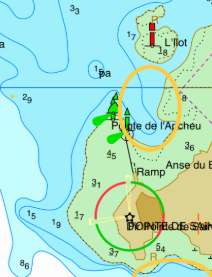
\includegraphics[height=\linewidth]{mouillage-st-gildas.png}
        \end{minipage}


\end{minipage}

%%%%%%%%%%%%%%%%%%%%
% Page de gauche n°2 
%%%%%%%%%%%%%%%%%%%%
\begin{minipage}[t][\textheight][t]{0.33\textwidth}
    \colorbox{StrongBlue}{
        \parbox[c][\textheight][c]{\textwidth}{ 
            \color{OffWhite} 
            \begin{center}
                \begin{minipage}[t][0.6\textheight][c]{0.8\textwidth}
                    \begin{center}
                        {\huge \textbf{Samedi 18 Juillet}}\\
                        {\huge \textbf{suite}}\\
                    \end{center}       
                \end{minipage}%
    
            \end{center}       
        }      
    }
\end{minipage}%
\begin{minipage}[c][\textheight][t]{0.10\textwidth}
\hfill
\end{minipage}%
\begin{minipage}[c][\textheight][t]{0.50\textwidth}
    \vspace{2.5cm}
    \color{StrongBlue}    
    {\huge \textbf{Suite de la description de la navigation}}\\
    \vspace{0.1cm}\\
    {\large \textbf{Traversée, suite}}\\
        \begin{itemize}
                \itemsep0em 
                \item Départ du mouillage
                \item Cap au 200°, direction la pointe de Noirmoutier
                \item Laisser la cardinale Nord Banc de la Blanche sur notre bâbord et se diriger vers la basse de Mortroger
                \item Affaler devant le port, avant tourelle Nord La Basse du Martroger à laisser sur bâbord
        \end{itemize}
    {\large \textbf{Entrée a L'Herbaudière}}\\
        \begin{minipage}[c]{0.65\textwidth}
        \begin{itemize}
                \itemsep0em 
                \item Le port de l'Herbaudière comporte un chenal d'accès qui nécessite de suivre un allignement de deux feux (en jaune sur la carte).
                \item Bien suivre l'allignement et le chenal, surtout à marée basse même si nous arriverons et partirons à mi-marée.
                \item Bien longer les latérales tribord pour éviter La Potée de Beurre tout en continuant de suivre l’alignement. 
                \item Un bateau CF devant et un derrière pour s'assurer que tout le monde suit l'allignement.
                \item Le port est accessible par tout temps et abrité de tout vent.
        \end{itemize}
        \end{minipage}
        \hfill
        \begin{minipage}[c]{0.30\textwidth}
                \centering
                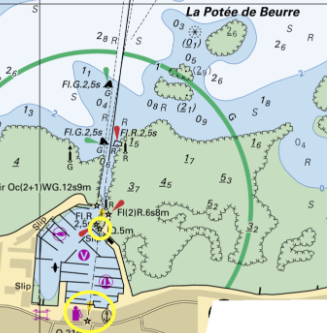
\includegraphics[height=\linewidth]{herbaudière-accès.png}
        \end{minipage}   
\end{minipage}%

%%%%%%%%%%%%%%%%
% Page de droite 1
%%%%%%%%%%%%%%%%
\newgeometry{top=2cm, bottom=2cm, left=2cm, right=2cm}
\begin{minipage}[t][0.9\textheight][t]{0.60\textwidth}
    \color{StrongBlue}    
    \noindent
    \begin{minipage}[t][0.3\textheight][t]{\textwidth}
        \begin{minipage}[t][0.3\textheight][t]{0.65\textwidth}
            \vspace{-8.5em}
            {\huge \textbf{Détails de la navigation}}\\
            Le QR-code situé à droite est cliquable, il permet d'explorer le planning de navigation sur le site datashom. 
            La carte ci-dessous visualise le trajet prévu ainsi que les abris de replis et dangers identifiés. 
        \end{minipage}%
        \hfill
        \begin{minipage}[t][0.3\textheight][t]{0.25\textwidth}       
        \href{https://data.shom.fr/datacontext/fr/1780656173959-146138}{ 
            
\includegraphics[width=0.8\textwidth]{qr-code.png}
        }
        \end{minipage}%
    \end{minipage}
    \begin{minipage}[t][0.7\textheight][t]{\textwidth}
        % 
\includegraphics[width=0.97\textwidth]{carte.png}
        
\includegraphics[height=0.7\textheight]{carte.png}
    \end{minipage}
\end{minipage}
\begin{minipage}[t][0.9\textheight][t]{0.40\textwidth}
    \color{StrongBlue} 
    \centering 
    
\includegraphics[height=\textheight, width=\textwidth, keepaspectratio]{illustration_verticale.jpg}
\end{minipage}%
\restoregeometry

%%%%%%%%%%%%%%%%
% Page de droite 2
%%%%%%%%%%%%%%%%
\newgeometry{top=1cm, bottom=2cm, left=1cm, right=1cm}
\begin{minipage}[c][0.9\textheight][t]{\textwidth}
    \color{StrongBlue}    
    \noindent
    \centering 
    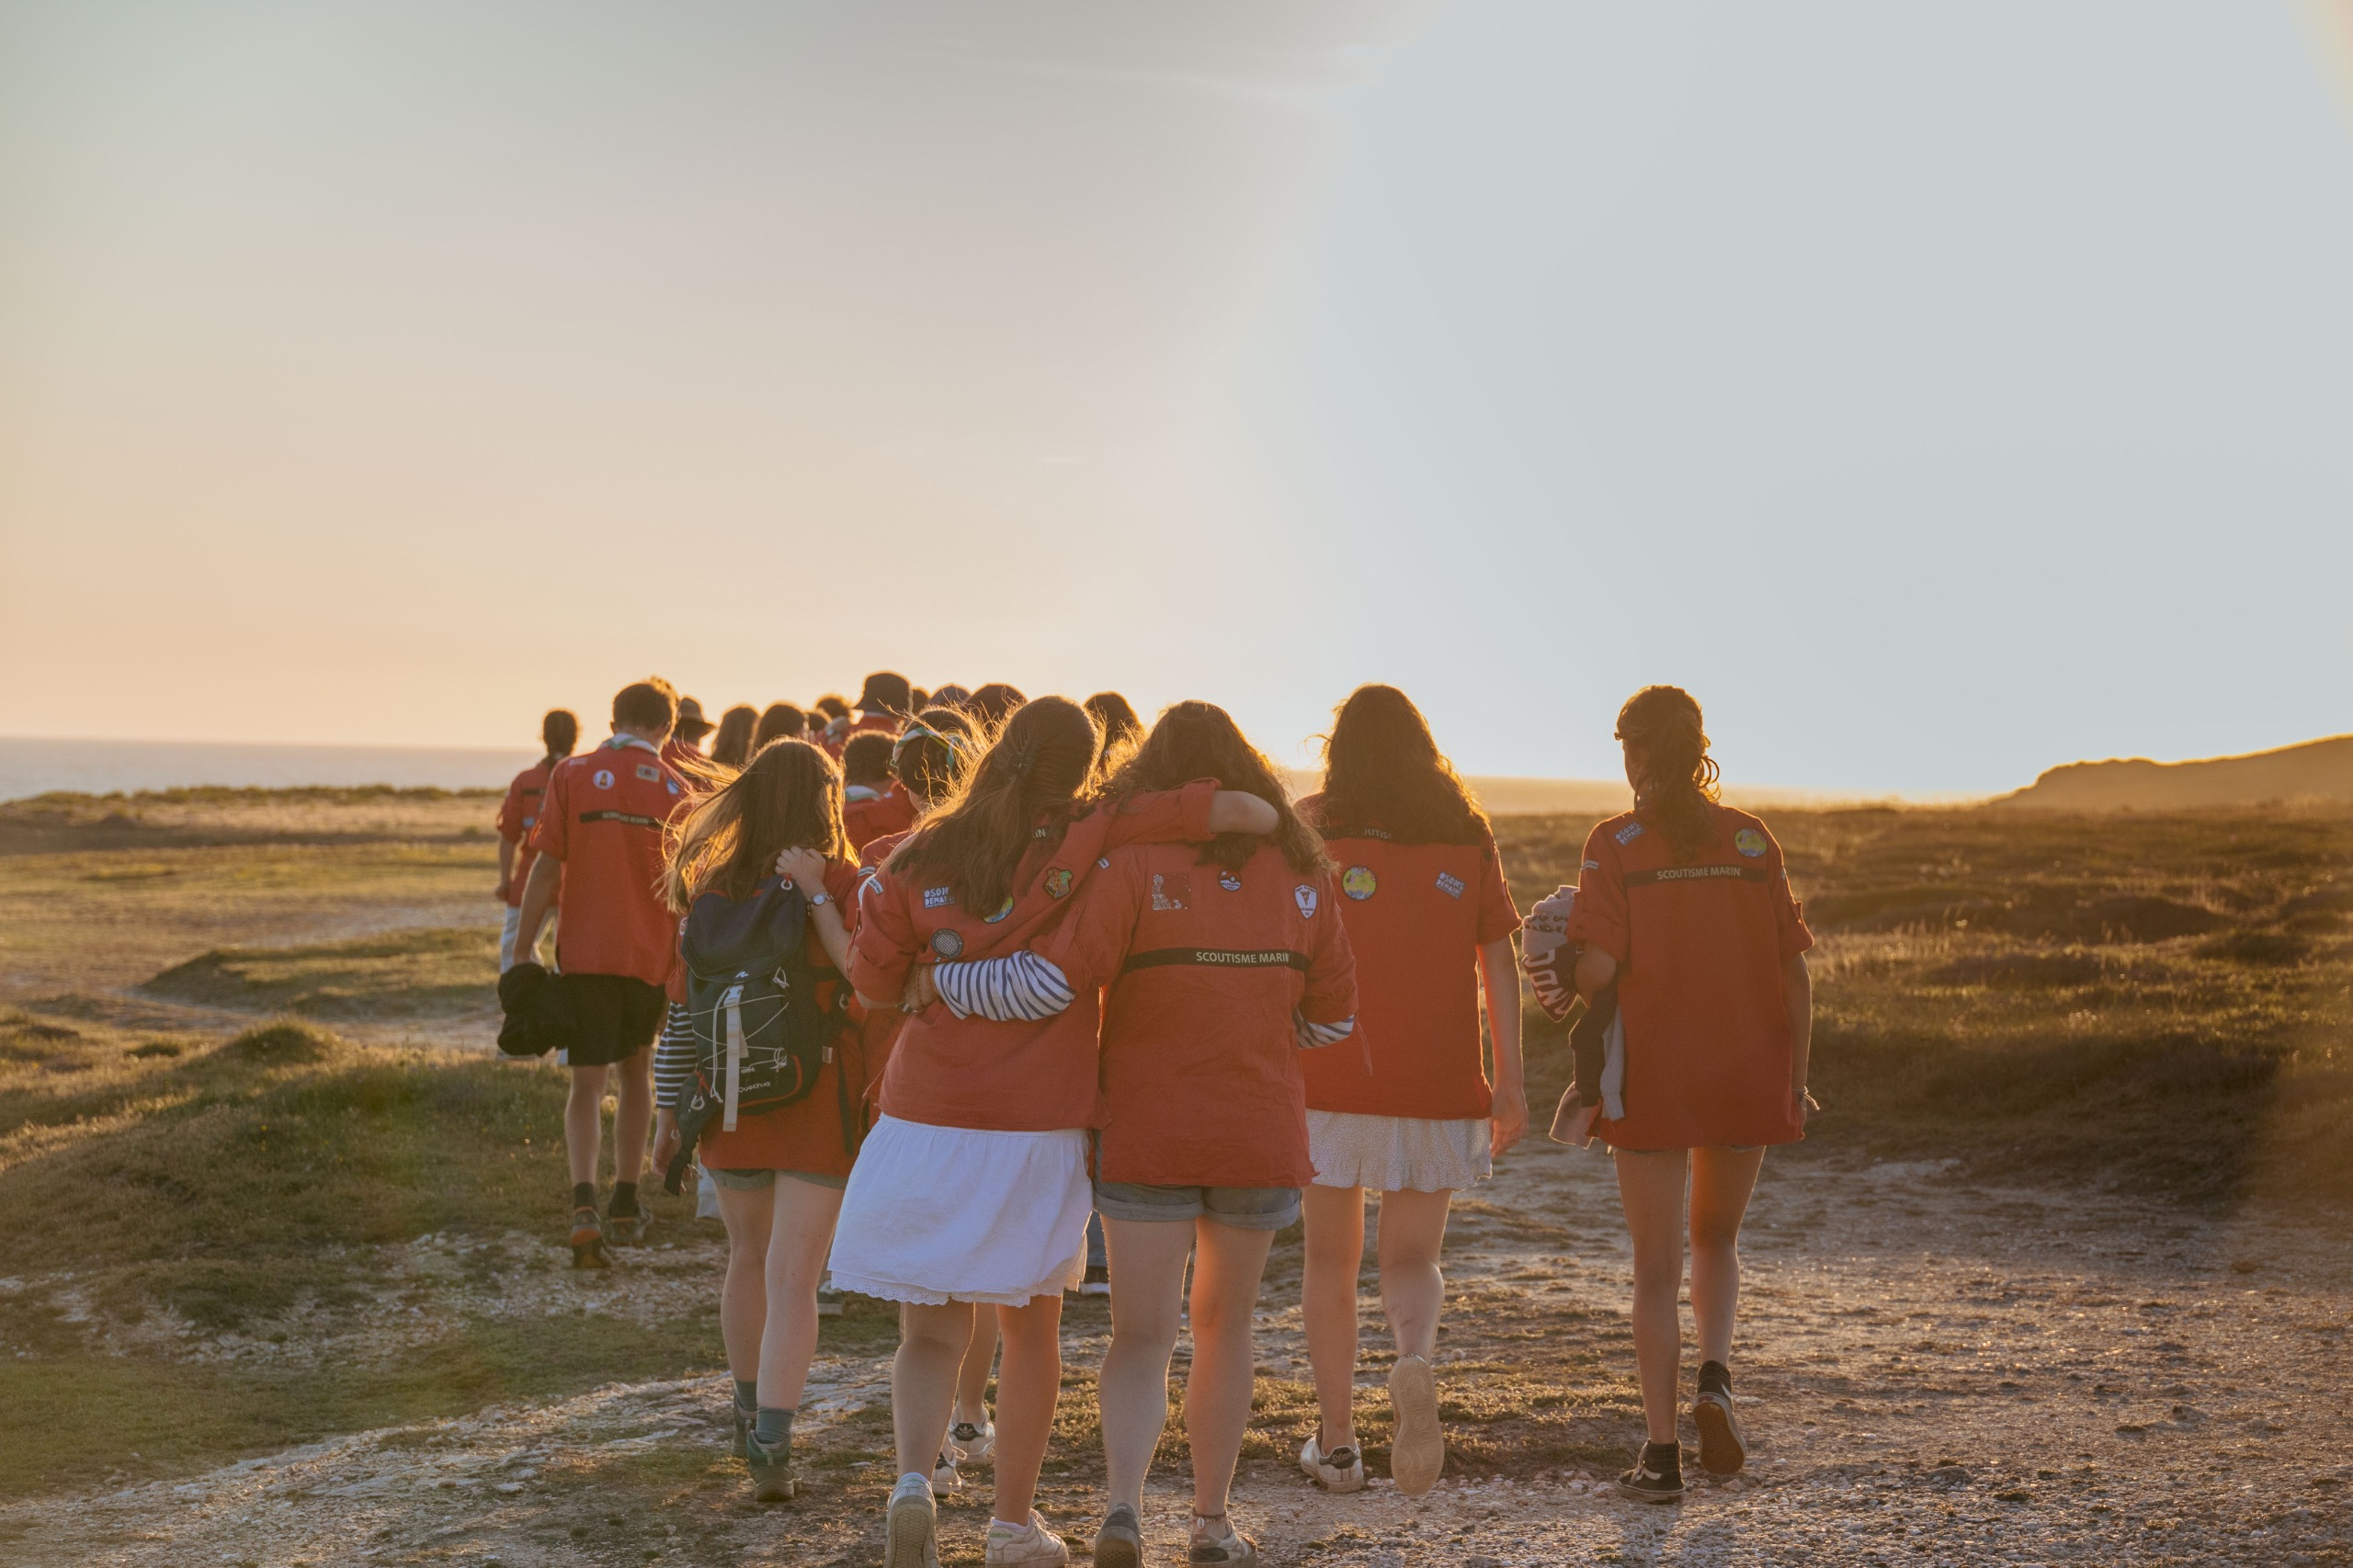
\includegraphics[height=\textheight, width=\textwidth, keepaspectratio]{Templates/horizontal_2.jpeg}
\end{minipage}%
\restoregeometry




